\documentclass{article}

\usepackage{fancyhdr}
\usepackage{extramarks}
\renewcommand{\thispagestyle}[1]{} % damit Titelseite Kopfzeile bekommt
\usepackage{amsmath}
\usepackage{amsthm}
\usepackage{amsfonts}
\usepackage{tikz}
\usepackage[plain]{algorithm}
\usepackage{algpseudocode}
\usepackage{listings}
\lstset{language=C++, numbers=left, frame=single,}
\usepackage[utf8]{inputenc}
\usepackage{paralist}
\usepackage{multicol}
\usepackage{amssymb}
\usepackage{mathtools}
\usepackage{a4wide}
\usepackage{color}
\usetikzlibrary{arrows}
\usepackage{stmaryrd}
\usepackage{relsize}
\usepackage{qtree}


\usetikzlibrary{automata,positioning}

%
% Basic Document Settings
%

\topmargin=-0.45in
\evensidemargin=0in
\oddsidemargin=0in
\textwidth=6.5in
\textheight=9.0in
\headsep=0.25in

\linespread{1.1}

\pagestyle{fancy}
\lhead{\hmwkGroup\\\hmwkTitle}
\rhead{\hmwkAuthorName}
\lfoot{\lastxmark}
\cfoot{\thepage}

\renewcommand\headrulewidth{0.4pt}
\renewcommand\footrulewidth{0.4pt}

\setlength\parindent{0pt}

%
% Create Problem Sections
%

\newcommand{\enterProblemHeader}[1]{
    \nobreak\extramarks{}{Aufgabe \arabic{#1} wird auf nächster Seite fortgesetzt\ldots}\nobreak{}
    \nobreak\extramarks{Aufgabe \arabic{#1} (fortgesetzt)}{Aufgabe \arabic{#1} wird auf nächster Seite fortgesetzt\ldots}\nobreak{}
}

\newcommand{\exitProblemHeader}[1]{
    \nobreak\extramarks{Aufgabe \arabic{#1} (fortgesetzt)}{Aufgabe \arabic{#1} wird auf nächster Seite fortgesetzt\ldots}\nobreak{}
    \stepcounter{#1}
    \nobreak\extramarks{Aufgabe \arabic{#1}}{}\nobreak{}
}

\setcounter{secnumdepth}{0}
\newcounter{partCounter}
\newcounter{homeworkProblemCounter}
\setcounter{homeworkProblemCounter}{1}
\nobreak\extramarks{Aufgabe \arabic{homeworkProblemCounter}}{}\nobreak{}

%
% Homework Problem Environment
%
% This environment takes an optional argument. When given, it will adjust the
% problem counter. This is useful for when the problems given for your
% assignment aren't sequential. See the last 3 problems of this template for an
% example.
%

\newenvironment{homeworkProblem}[1][-1]{
    \ifnum#1>0
        \setcounter{homeworkProblemCounter}{#1}
    \fi
    \section{Aufgabe \arabic{homeworkProblemCounter}}
    \setcounter{partCounter}{1}
    \enterProblemHeader{homeworkProblemCounter}
}{
    \exitProblemHeader{homeworkProblemCounter}
}

%
% Homework Details
%   - Title
%   - Due date
%   - Class
%   - Section/Time
%   - Instructor
%   - Author
%

\date{22.6.2018}
\newcommand{\hmwkTitle}{Übungsblatt\ \#9}
\newcommand{\hmwkGroup}{Übungsgruppe 16}
\newcommand{\hmwkDueDate}{28. Juni 2018}
\newcommand{\hmwkClass}{Datenstrukturen und Algorithmen}
\newcommand{\hmwkAuthorName}{\textbf{Finn Hess (378104), Jan Knichel (377779), Paul Orschau (381085)}}

%
% Title Page
%

\title{
    \vspace{2in}
    \textmd{\textbf{\hmwkClass:\ \hmwkTitle}}\\
    \normalsize\vspace{0.1in}\small{Abgabe\ am\ \hmwkDueDate\ }\\
    \vspace{3in}
}

\author{\hmwkAuthorName}

\renewcommand{\part}[1]{\textbf{\large Part \Alph{partCounter}}\stepcounter{partCounter}\\}

%
% Various Helper Commands
%

% Useful for algorithms
\newcommand{\alg}[1]{\textsc{\bfseries \footnotesize #1}}

% For derivatives
\newcommand{\deriv}[1]{\frac{\mathrm{d}}{\mathrm{d}x} (#1)}

% For partial derivatives
\newcommand{\pderiv}[2]{\frac{\partial}{\partial #1} (#2)}

% Integral dx
\newcommand{\dx}{\mathrm{d}x}

% Alias for the Solution section header
\newcommand{\loesung}{\textbf{\large Lösung}}

% Parts
\newcommand{\teil}[1]{\vspace{15pt}\textbf{Teil #1}}


%
% Start of Document
%

\begin{document}

  \maketitle

  \pagebreak
  
  \begin{homeworkProblem}
    
    \teil{a)}  
\\ Gerichtete Graphen mit $n \in \mathbb{N}$ Knoten:
\\ Die Adjazenzmatrix ist also eine $n \times n$  Matrix, in der jeder Eintrag $0$ oder $1$ ist.
\\ Es gibt also $n \cdot n = n^2$ Werte mit je zwei M\"oglichkeiten.
$$\Rightarrow 2^{(n^2)}$$

    \teil{b)}
\\ Ungerichtete Graphen mit $n \in \mathbb{N}$ Knoten:
\\ Die Adjazenzmatrix eine symmetrische $n \times n$ Matrix, wobei auf der Diagonalen nur Nulleintr\"age sind (keine Kanten von $i$ nach $i$ f\"ur $ i \in n$)
\\ Es gibt also $n \cdot n = n^2$ Werte. Von diesen Werten sind $n$ Nullwerte auf der Diagonalen vorgegeben. Von den $n^2-n$ verbliebenen Werten ist aufgrund der Symmetrie nur die H\"alfte frei w\"ahlbar, also $\frac{n^2-n}{2}$ Werte mit je zwei M\"oglichkeiten.
$$\Rightarrow 2^{\frac{n^2-n}{2}}$$

    \teil{c)}
\\ einfache Pfade der L\"ange $k$ f\"ur vollst\"andig ungerichtete Graphen:
\\$k=0:$ $n$ Pfade (entspricht Anzahl der Knoten)
\\ $k=1:$ $\frac{n(n-1)}{2}$ Pfade (entspricht Anzahl Kanten: jeder Knoten hat $(n-1)$ Kanten 
\\$\Rightarrow$ Kanten gesamt: $\sum_{i=1}^{n-1} i$)
\\ $k \geq 2:$ Es gibt $n$ m\"ogliche Startknoten mit $n-1$ Nachfolgern. Da nur nach einfachen Pfaden gesucht wird, bleiben danach nur $n-2$ M\"oglichkeiten usw.
$$\Rightarrow \prod_{i=0}^{k} (n-i)$$

    \teil{d)}
\\ Zykel der L\"ange h\"ochstens $4$ f\"ur vollst\"andig ungerichtete Graphen:
\\Zykel in ungerichteten Graphen haben laut Definition mindestens die L\"ange drei.
\\\textit{L\"ange $3$:}
\\ $n$ m\"ogliche Startpositionen mit je $n-1$ Nachfolgern. Da die Knoten paarweise verschieden sein m\"ussen, gibt es danach noch $n-2$ M\"oglichkeiten. Danach muss die Kante zum Startknoten gew\"ahlt werden.
\\ $\Rightarrow n(n-1)(n-2)$
\\\textit{L\"ange $4$:}
\\Nach den $n-2$ m\"oglichen Knoten gibt es im n\"achsten Schritt $n-3$ m\"ogliche Nachfolger, da von den $n-1$ Nachbarknoten zwei ausgeschlossen sind: der Vorg\"angerknoten und der Startknoten.
\\Danach muss zum Startknoten zur\"uckgegangen werden.
\\ $\Rightarrow n(n-1)(n-2)(n-3)$
$$ \Rightarrow n(n-1)(n-2)+n(n-1)(n-2)(n-3) = n(n-1)(n-2)^2$$

\newpage

    \teil{e)}
\\ (i) $\hat{G}$ symmetrisch:
\\F\"ur $(u,v) \in E$ gilt per Definition f\"ur transponierte Graphen:
$$ (u,v) \in E \Leftrightarrow (v,u) \in E'$$
Mit $\hat{E} = E \cup E'$ gilt $(u,v) \in \hat{E}$ und $(v,u) \in \hat{E}$
\\Das beinhaltet die Definition f\"ur Symmetrie: $(u,v) \in \hat{E} \Rightarrow (v,u) \in \hat{E}$
$$ $$
(ii) $\hat{G}$ stark zusammenh\"angend $\Rightarrow$ $G$ oder $G^{T}$ stark zusammenh\"angend:
\\Gegenbeispiel,  $\hat{G}$ stark zusammeng\"angend:
$$ $$
$G$ nicht stark zusammeng\"angend:
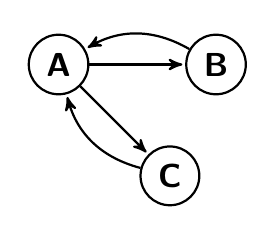
\begin{tikzpicture}[->,>=stealth',shorten >=1pt,auto,node distance=2cm,
                    thick,main node/.style={circle,draw,font=\sffamily\large\bfseries}]

  \node[main node] (1) {A};
  \node[main node] (2) [right of=1] {B};
  \node[main node] (3) [below right of=1] {C};

  \path[every node/.style={font=\sffamily\small}]
    (1) edge node  {} (2)
        edge node  {} (3)
    (2) edge [bend right] node   {} (1)
    (3) edge [bend left] node  {} (1);

\end{tikzpicture}
\\$G^{T}$ nicht stark zusammenh\"angend:
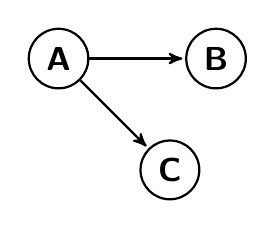
\begin{tikzpicture}[->,>=stealth',shorten >=1pt,auto,node distance=2cm,
                    thick,main node/.style={circle,draw,font=\sffamily\large\bfseries}]

  \node[main node] (1) {A};
  \node[main node] (2) [right of=1] {B};
  \node[main node] (3) [below right of=1] {C};

  \path[every node/.style={font=\sffamily\small}]
    (1) edge node {} (2)
        
    (1) edge node {} (3);
\end{tikzpicture}
\\ $\Rightarrow$(ii) gilt nicht.$\;\;\;\;\;\;\;\;\;\;\;\;\;\;\;\;\;\;\;\;\;\;\;\;\;\;\;\;\;\;$
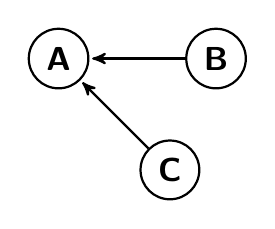
\begin{tikzpicture}[->,>=stealth',shorten >=1pt,auto,node distance=2cm,
                    thick,main node/.style={circle,draw,font=\sffamily\large\bfseries}]

  \node[main node] (1) {A};
  \node[main node] (2) [right of=1] {B};
  \node[main node] (3) [below right of=1] {C};

  \path[every node/.style={font=\sffamily\small}]
    (2) edge node {} (1)
        
    (3) edge node {} (1);
\end{tikzpicture}
$$ $$
(iii)  $G$ oder $G^{T}$ stark zusammenh\"angend $\Rightarrow$ $\hat{G}$ stark zusammenh\"angend:
\\Durch die Menge der Kanten $E$ oder $E'$ sind per Voraussetzung schon alle Knoten von jedem anderen beliebigen Knoten erreichbar. Da $\hat{E}$ die Vereinigung der beiden Kantenmengen darstellt und die Knoten in $\hat{G}$ die gleichen wie in $G$ und $G^{T}$ sind, m\"ussen in $\hat{G}$ also auch alle Knoten erreichbar sein, $\hat{G}$ ist also stark zusammenh\"angend.
$$ $$
(iv) $G$ schwach zusammenh\"angend $\Leftrightarrow$ $G^{T}$ schwach zusammenh\"angend:
\\Bei der Eigenschaft "schwach zusammenh\"angend" werden die Graphen als ungerichtete Graphen betrachtet, die Pfeilrichtungen werden als ignoriert. Da durch das Transponieren nur die Pfeilrichtungen vertauscht werde, gilt: $G_{ungerichtet} = G_{ungerichtet}^{T}$. 
Die beiden ungerichteten Graphen sind also gleich, daher gilt insbesondere, dass immer beide oder keiner stark zusammenh\"angend ist, also f\"ur die gerichteten Graphen:
\\$G$ und $G^{T}$ sind entweder beide schwach zusammenh\"angend oder keiner ist es.
\\ Folglich: $G$ schwach zusammenh\"angend $\Leftrightarrow$ $G^{T}$ schwach zusammenh\"angend.

\newpage

    \teil{f)}
\\ Jeder knotengewichtete DAG hat genau einen kritischen Pfad.
\\ Der kritische Pfad ist der l\"angste Pfad (bezogen auf das Gesamtgewicht) im DAG und startet bei einem Knoten $v_{0}$ ohne Abh\"angigkeiten.
Falls es ein eindeutiges Maximum $eft(v_{k})$ gibt, stimmt die Aussage.
Dies muss allerdings nicht der Fall sein, wenn z.B. zwei Knoten gleich gewichtet sind:
$$ $$
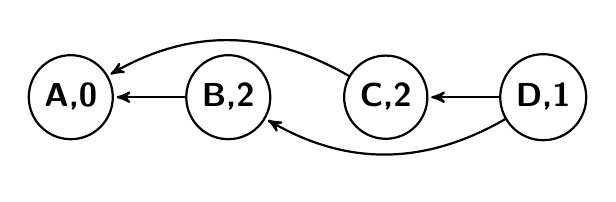
\begin{tikzpicture}[->,>=stealth',shorten >=1pt,auto,node distance=2cm,
                    thick,main node/.style={circle,draw,font=\sffamily\large\bfseries}]

  \node[main node] (1) {A,0};
  \node[main node] (2) [right of=1] {B,2};
  \node[main node] (3) [right of=2] {C,2};
  \node[main node] (4) [right of=3] {D,1};
  \path[every node/.style={font=\sffamily\small}]
    (2) edge node {} (1)
    (3) edge [bend right] node {} (1)
    (4) edge [bend left] node {} (2)
    (4) edge node {} (3);
\end{tikzpicture}
\\Kritischer Pfad 1: 
$$ A = v_{0},\;\; B = v_{1},\;\; D = v_{2},\;\; eft(v_{2}) = 3$$
Kritischer Pfad 2:
$$ A = v_{0},\;\; C = v_{1},\;\; D = v_{2},\;\; eft(v_{2}) = 3$$
$$ $$

  \end{homeworkProblem}

  \begin{homeworkProblem}[2]
    
    \teil{a)}

    \textbf{These:} Die Funktion \texttt{DFS(...)} wird auf jeden der $n$ Knoten genau einmal ausgeführt.
    
    \textbf{Beweis:} Am Anfang sind offensichtlich alle Knoten \textbf{weiß} gefärbt (Zeile 16) und am Ende alle \textbf{schwarz}. Eine komplette Tiefensuche findet alle Knoten, selbst wenn es gar keine Kanten gibt, da die \texttt{for}-Schleife in Zeile 17 alle Knoten \textbf{mindestens einmal} prüft und ggf. \texttt{DFS(...)} \textbf{mindestens einmal} ausführt. Da vor den beiden Aufrufen von \texttt{DFS(...)} in den Zeilen 7 und 19 jeweils die Farbe des Knotens überprüft wird, kann die Funktion \textbf{nicht öfter als einmal} pro Knoten ausgeführt werden, denn \texttt{DFS(...)} färbt jeden Knoten sofort grau (Zeile 3) und verhindert somit, dass ein Knoten doppelt besucht wird.
    
    \textbf{Folgerung:} Zeilen 2, 3, 11, 12 liegen in $\Theta(n)$.
    
    \vspace{0.2in}
    
    Da die \texttt{for}-Schleife in Zeile 4 für jeden Knoten, also für jedes $n$, genau einmal erreicht wird, liegen Zeilen 4 und 5 in $\Theta(n^2)$. Jeder Eintrag der Adjazenzmatrix wird also genau einmal überprüft, und abhängig von der Anzahl von \texttt{true} Werten, also der Anzahl der Kanten $m$, wird Zeile 6 ausgeführt, sie liegt also in $\Theta(m)$. Da aber gilt $m \leq n^2$ kann diese Zeile die asymptotische Laufzeit nicht weiter verschlechtern, ausschlaggebend sind also weiterhin Zeilen 4 und 5.
    
    Insgesamt gilt also:

    \begin{equation}
      T(n,m) \in \Theta(n^2)
    \end{equation}
    
    \teil{b)}
    
    Siehe Begründung der a), alle \texttt{print(...)} Anweisungen stehen in der \texttt{DFS(...)} Funktion, welche genau $n$-mal ausgeführt wird, somit gilt:
    
    \begin{equation}
      T(n,m) = 2n \in \Theta(n)
    \end{equation}
    
  \end{homeworkProblem}

  \begin{homeworkProblem}
    
    \textbf{SCCs in gerichteten Graphen}
    
    \teil{a)}
    
    w= white, g=grey, b=black
    $$ $$
    \begin{tabular}{c c c c c c c c c c c c }
    	1. Phase  & 1 & 2 & 3 & 4 & 5 & 6 & 7 & 8 & 9 & 10 & 11 \\
    	1: color & b & w & w & b & b & b & b & b & b & b & b \\
    	S		 & 4 & 11 & 8 & 9 & 10 & 7 & 6 & 5 & 1 \\
    			 & & & & & & & & & \\
    	2: color & b & b & b & b & b & b & b & b & b & b & b \\
    	S		 & 4 & 11 & 8 & 9 & 10 & 7 & 6 & 5 & 1 & 3 & 2 \\
    \end{tabular}
    $$ $$
    \begin{tabular}{c c c c c c c c c c c c }
    	2.Phase  & 1 & 2 & 3 & 4 & 5 & 6 & 7 & 8 & 9 & 10 & 11 \\
    	1: color & w & b & b & w & w & w & w & w & w & w & w \\
    	S		 & 4 & 11 & 8 & 9 & 10 & 7 & 6 & 5 & 1 & 3\\
    	Suc		 & 0 & 2 & 2 & 0 & 0 & 0 & 0 & 0 & 0 & 0 & 0 \\
    			 & & & & & & & & & \\
    	2: color & b & b & b & w & b & b & b & b & b & b & b \\
    	S		 & 4 & 11 & 8 & 9 & 10 & 7 & 6 & 5 \\
    	Suc		 & 1 & 2 & 2 & 0 & 1 & 1 & 1 & 1 & 1 & 1 & 1 \\
    			 & & & & & & & & & \\
    	3: color & b & b & b & b & b & b & b & b & b & b & b \\
    	S		 & & & & & & & & & \\
    	Suc		 & 1 & 2 & 2 & 4 & 1 & 1 & 1 & 1 & 1 & 1 & 1 \\
    \end{tabular}
    $$ $$
    
    \teil{b)}
    
    Kondensationsgraph:
    \\ A: 1,5,6,7,8,9,10,11
    \\ B: 2,3
    \\ C: 4
    $$ $$
    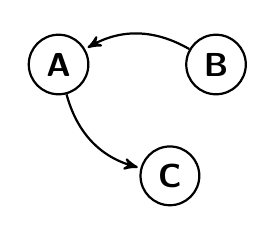
\begin{tikzpicture}[->,>=stealth',shorten >=1pt,auto,node distance=2cm,
                        thick,main node/.style={circle,draw,font=\sffamily\large\bfseries}]

      \node[main node] (1) {A};
      \node[main node] (2) [right of=1] {B};
      \node[main node] (3) [below right of=1] {C};
      \path[every node/.style={font=\sffamily\small}]
        (2) edge [bend right] node {} (1)
        (1) edge [bend right] node {} (3);
        
    \end{tikzpicture}
    
  \end{homeworkProblem}
  
  \pagebreak

  \begin{homeworkProblem}
    
    \teil{a)}
    
    \begin{tabular}{|c|c|c|c|c|c|c|c|c|c|c|c|c|c|c|c|c|c|c|c|c|}
      \hline
      	topo($v$) & 1 & 2 & 3 & 4 & 5 & 6 & 7 & 8 & 9 & 10 & 11 & 12 & 13 & 14 & 15 & 16 & 17 & 18 & 19 & 20 \\
      \hline
      	Knoten $v$ & 2 & 1 & 16 & 15 & 8 & 9 & 13 & 14 & 7 & 10 & 12 & 17 & 4 & 6 & 11 & 19 & 3 & 20 & 5 & 18 \\
      \hline
    \end{tabular}

    \teil{b)}
    
    \lstinputlisting{Code/4.cpp}
    
  \end{homeworkProblem}
  
  \pagebreak
  
  \begin{homeworkProblem}
    
    \begin{tabular}{c c c c c c c c c c c c c c c}
    	Knoten & A & B & C & D & E & F & G & H & I & J & K & L & M & N \\ 
    	est	   & 16 & 11 & 10 & 8 & 13 & 3 & 6 & 6 & 0 & 4 & 0 & 0 & 0 & 0 \\
    	critDep & E & G & D & F & C & M & J & L & -1 & N & -1 & -1 & -1 & -1 \\
    	eft	   & 20 & 13 & 13 & 10 & 16 & 8 & 11 & 9 & 3 & 6 & 3 & 6 & 3 & 4 \\	
    \end{tabular}
    $$ $$
    Schwarzf\"arbung: N,J,G,B,M,F,K,D,I,C,L,H,E,A
    \\Kritischer Pfad: A $\rightarrow$ E $\rightarrow$ C $\rightarrow$  D $\rightarrow$ F $\rightarrow$ M
    \\Gesamtdauer: 20
    
  \end{homeworkProblem}
  
  \begin{homeworkProblem}
    
    \lstinputlisting{Code/6.cpp}
    
    Die Funktion basiert auf der Breitensuche. Wir gehen von einem zusammenh\"angenden Graphen aus.
    \\Die Korrektheit der Funktion besteht darin, dass alle durch eine Kante verbundenen Knoten abwechselnd rot und schwarz gef\"arbt werden. So werden sie jeweils einer Menge $U$ und $W$ zugeordnet.
    \\Dass keine Kanten innerhalb dieser Mengen existieren, wird durch Abgleich der Farben gew\"ahrleistet. Haben zwei aufeinanderfolgende Knoten die gleiche Farbe, wird \texttt{false} zur\"uckgegeben.
    \\Da es sich um zusammenh\"angende Graphen handelt, wird durch die Breitensuche der gesamte Graph abgedeckt. 
    
  \end{homeworkProblem}

\end{document}